\paragraph{} The process of implementing the front-end from prototype to deployment is not only an exciting journey, but it is also a process filled with valuable learning experiences for our development team. During this phase, we have acquired new knowledge and skills while fine-tuning and refining the project to ensure optimal performance and suitability. As a result, the official website has undergone several improvements and enhancements compared to the prototype version. In this section of the report, we will highlight the key areas where we have made significant improvements to the project.
\paragraph{}First and foremost, after the hero section, we showcase logos of major tech companies (Figure \ref{fig:logos}) that use our platform, helping build trust and credibility with potential users.
  \begin{figure}[h]
    \centering
    
\includegraphics[width= 1\textwidth]{figures/deploy_change.png}
     \caption{Company logos}
    \label{fig:logos}
\end{figure}
\paragraph{}We redesigned the "Why crypto?" section (see Figure \ref{fig:Why choose us}) to improve readability by adding more spacing between cards, making it more visually appealing than our previous layout. We added the headline "Trade crypto with confidence" to inspire trust and enthusiasm among potential users. We also made a deliberate choice to use "Why Choose Us?" (Figure \ref{fig:Why_choose_us_2.0}) instead of "Why crypto?"(see Figure \ref{fig:Why choose us}) as we believe this phrasing creates a more personal connection with users and emphasizes our community-focused approach, which helps build trust in our platform. We enhanced the section's key messages by using bolder, darker fonts that contrast well against the light background. This makes our core ideas immediately stand out and easier for users to grasp at first glance.
  \begin{figure}[h]
    \centering
    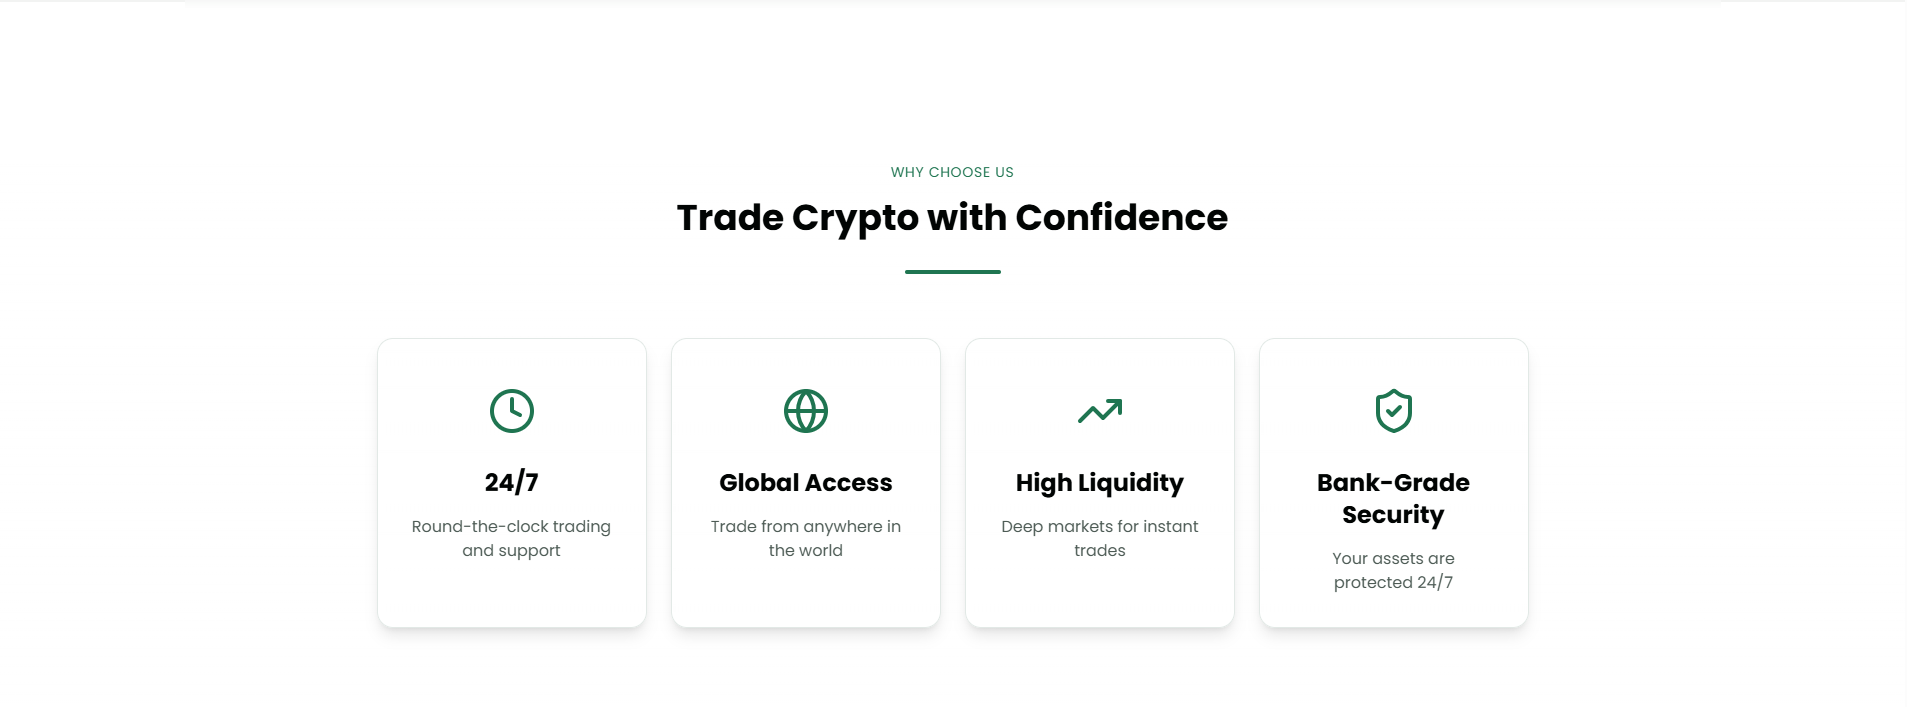
\includegraphics[width= 1\textwidth]{figures/deploy_change_2.png}
     \caption{Official Why choose us?}
    \label{fig:Why_choose_us_2.0}
\end{figure}
\paragraph{} In revamping the tutorial section, we moved away from our prototype's softer design (see Figure \ref{fig:step}) to better reflect cryptocurrency's cutting-edge nature, Figure \ref{fig:step_2.0}. We implemented a more modern aesthetic by using bold, dark backgrounds with white text, creating a sleek, tech-forward appearance. The instructions were also streamlined with shorter, more concise text to create a more user-friendly guide for newcomers.
  \begin{figure}[h]
    \centering
    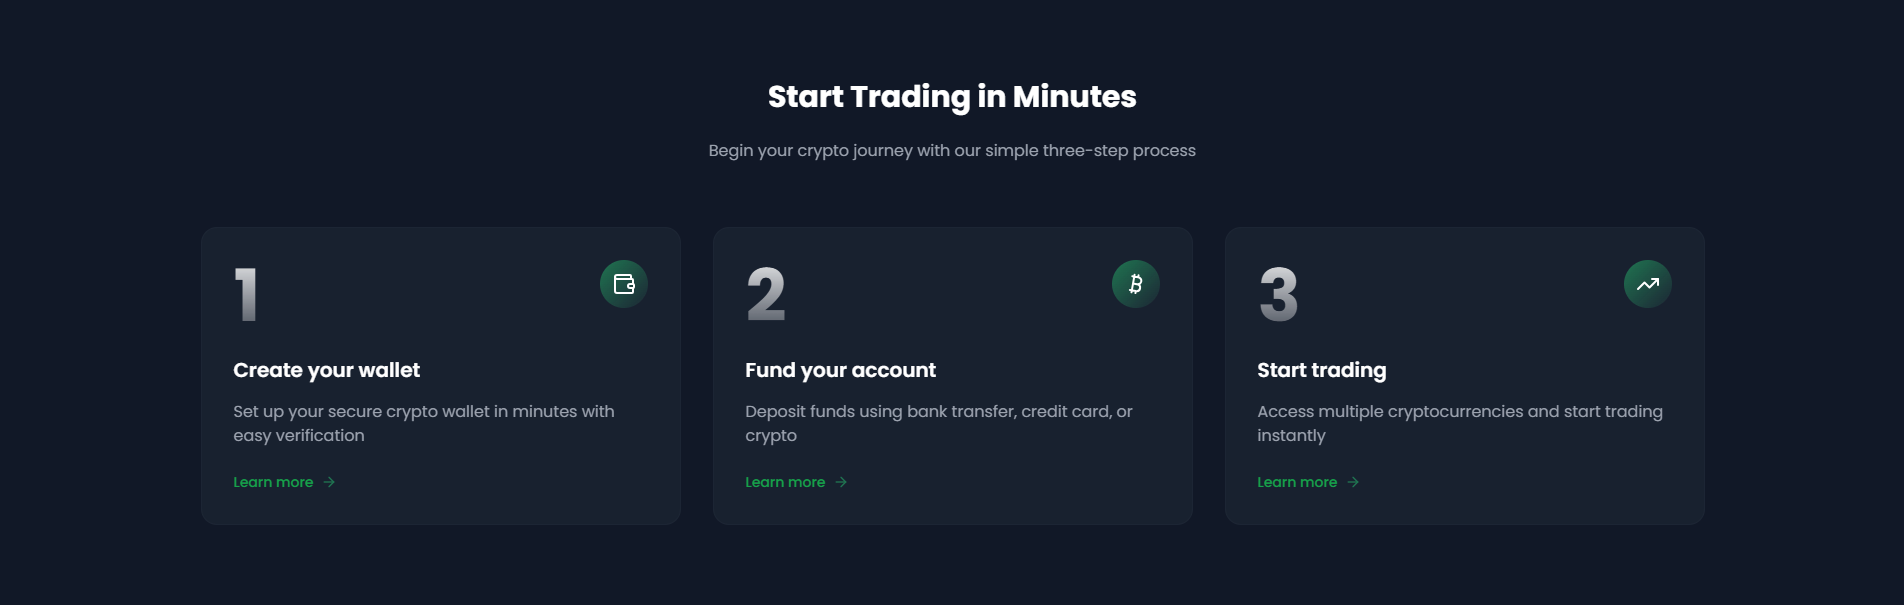
\includegraphics[width= 0.9\textwidth, keepaspectratio]{figures/Screenshot 2025-02-16 154618.png}
     \caption{Official Guide for users to start}
    \label{fig:step_2.0}
\end{figure}
\paragraph{}We simplified the mission section (see Figure \ref{fig:option}) by removing excess text and creating more white space. Instead, we now highlight key statistics about our platform's achievements, which demonstrate both our strong presence in the crypto trading community and our track record of consistent performance. This streamlined approach makes our success metrics more prominent and impactful. Those changed resulted in our new mission section, Figure \ref{fig:option_2.0}
  \begin{figure}[h]
    \centering
    
\includegraphics[width= 1\textwidth]{root/op1.png}
     \caption{Official Mission section}
    \label{fig:option_2.0}
\end{figure}
\paragraph{}We introduced a new free tier to our pricing structure to make our platform accessible to a wider range of users, from beginners to professional traders and organizations. Each pricing plan is carefully tailored to match different user needs and usage levels, ensuring that every customer segment finds an appropriate and cost-effective option for their trading activities.
  \begin{figure}[h]
    \centering
    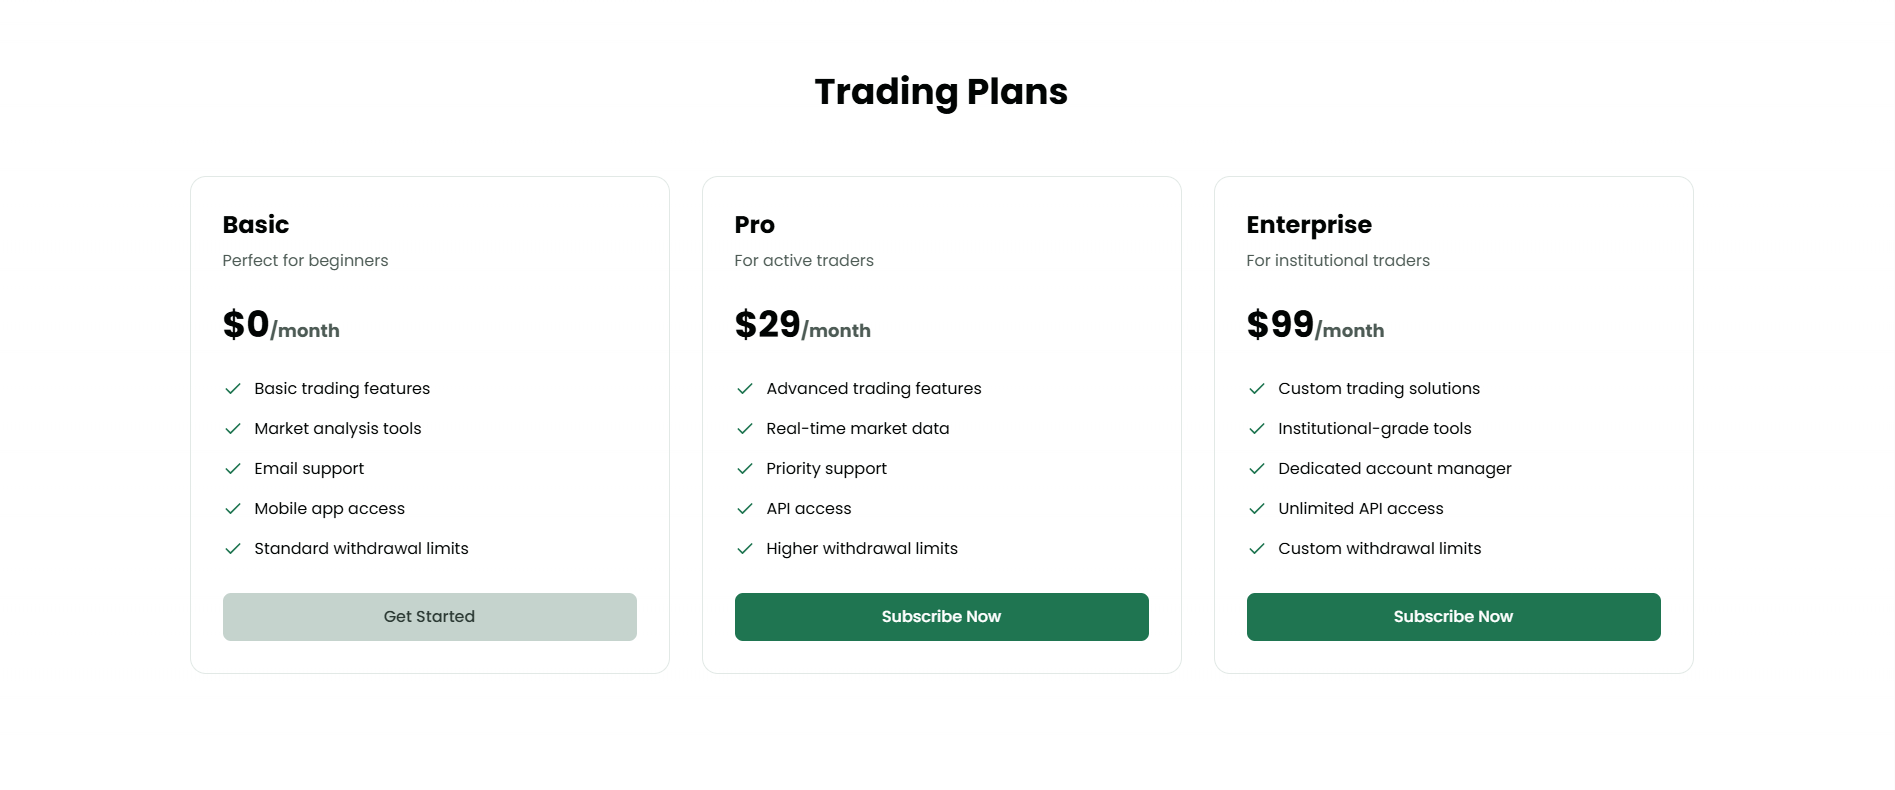
\includegraphics[width= 1\textwidth]{root/op2.png}
     \caption{Official Pricing Plan}
    \label{fig:option_2_2.0}
\end{figure}
\paragraph{} Lastly is our platform's "Try it out" section's transformation.The section underwent a complete strategic overhaul. Instead of focusing narrowly on payment processing for small businesses, we broadened our message to "Start Your Journey Today," positioning ourselves as a comprehensive global trading platform. To build credibility, we now showcase our key achievements: over \$2 billion in trading volume, operations in more than 180 countries, and a million-plus user base.
The design also evolved significantly, replacing the simple teal color scheme with a more sophisticated dark theme accented with green. We now prominently highlight crucial features like bank-grade encryption and high-speed transactions, addressing key user concerns about security and performance. The call-to-action button was also refined from a generic "Learn More" to a more action-oriented "View Pricing Plans," creating a clearer path for potential users.
 \begin{figure}[h]
    \centering
    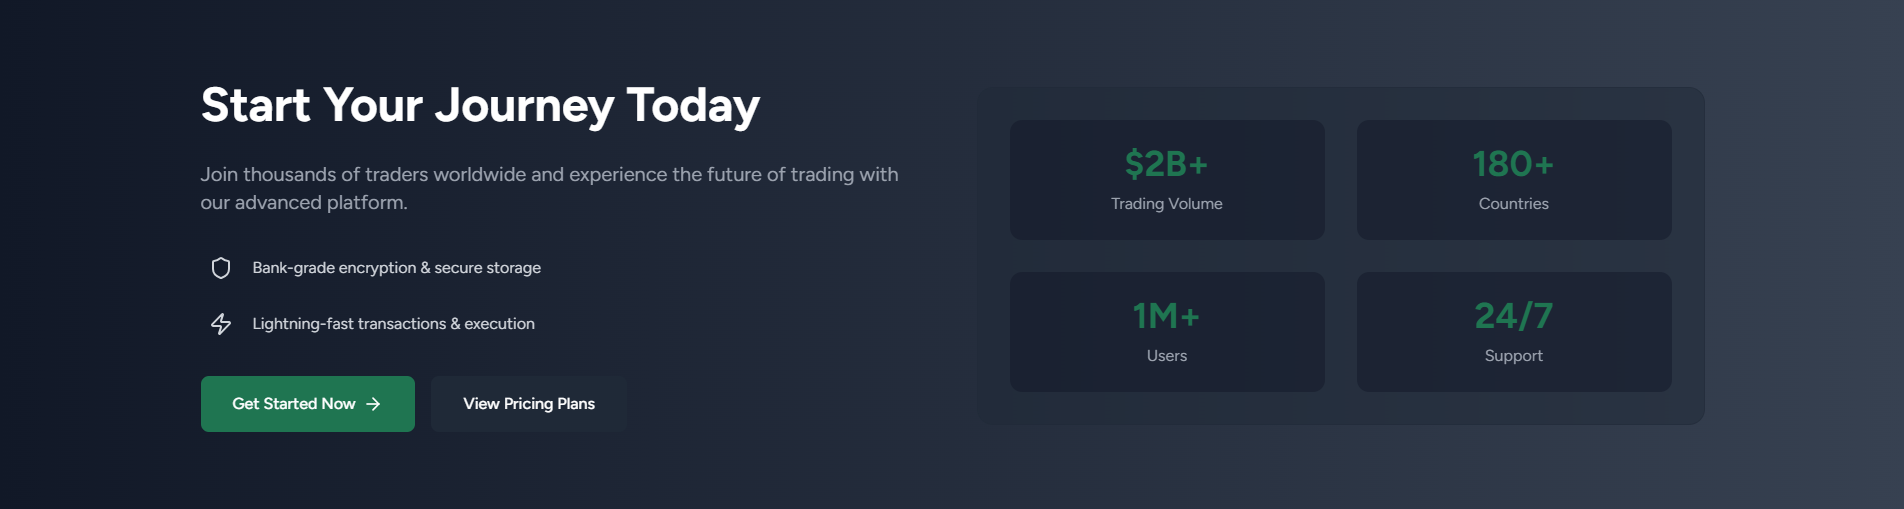
\includegraphics[width= 1\textwidth]{root/cta_2.png}
     \caption{Official Call-To-Action}
    \label{fig:cta_2.0}
\end{figure}
\paragraph{} The main component of my webpage is Wallets where users can keep track with their wallets' transaction information and activity. The search page of ./Wallets design stay unchanged compared to prototype, Figure \ref{fig:search}. Below the official search page:
 \begin{figure}[h]
    \centering
    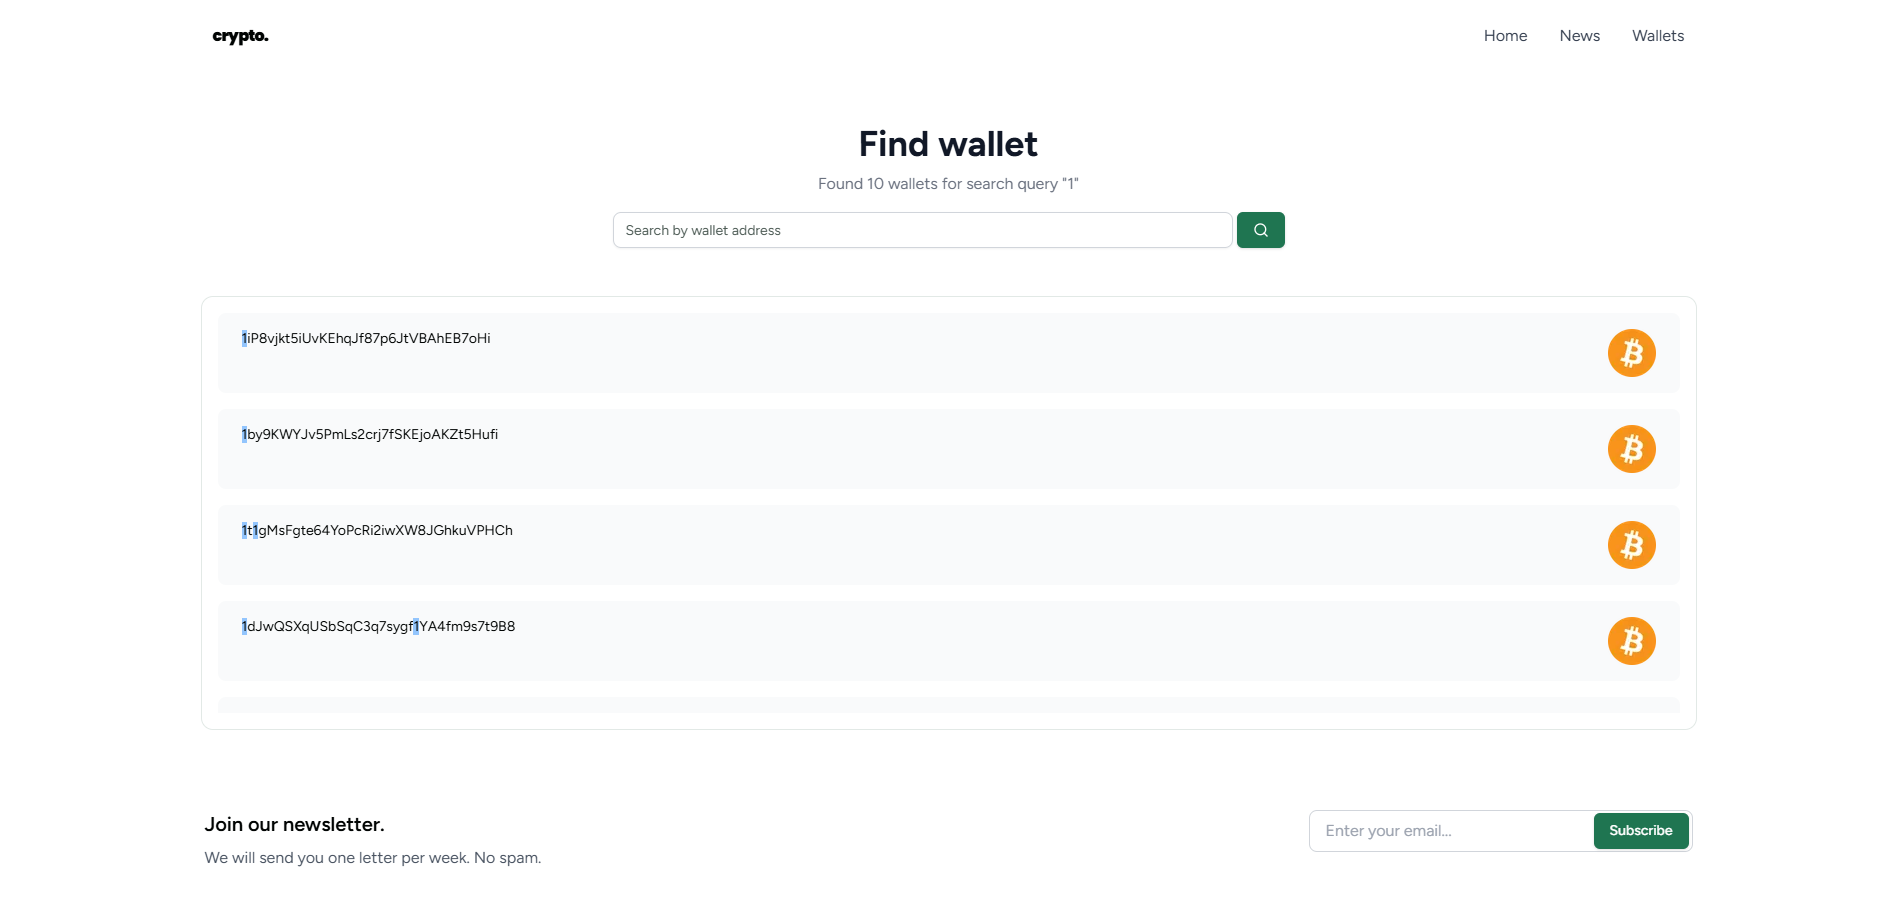
\includegraphics[width= 1\textwidth]{root/wallet_search.png}
     \caption{Official ./wallets}
    \label{fig:wallet_search}
\end{figure}
\paragraph{} The Wallet Details page (/wallets/:id/details) has been streamlined by removing the right panel that was intended to display a "Changes Over Time" line graph (refer to \ref{fig:Wallet_Detail}). This feature was removed because our team encountered significant implementation challenges and decided to postpone its development rather than delay the platform's launch. Similarly, the Transaction History page (/wallets/:id/history) has been simplified, with some transaction details being omitted from the original prototype to improve performance in this development phase.

\paragraph{} Throughout the development process, we have made strategic modifications to enhance performance and maintain consistency, resulting in some differences from our initial prototype. While certain features have been streamlined in this release, our team remains committed to advancing the platform's capabilities. We envision future iterations of our blockchain transaction visualization system incorporating more sophisticated features and technological breakthroughs, further enriching the user experience and functionality.



